\documentclass[conference]{IEEEtran}
\IEEEoverridecommandlockouts
\usepackage{cite}
\usepackage{amsmath,amssymb,amsfonts}
\usepackage{algorithmic}
\usepackage{graphicx}
\usepackage{textcomp}
\usepackage{xcolor}
\usepackage{url}
\def\BibTeX{{\rm B\kern-.05em{\sc i\kern-.025em b}\kern-.08em
    T\kern-.1667em\lower.7ex\hbox{E}\kern-.125emX}}

\begin{document}

\title{Towards Energy-Aware Design Choices in Event-Driven Microservices}

\author{\IEEEauthorblockN{Vijay}
\IEEEauthorblockA{\textit{Roll No. 2023111007} \\
\textit{IIIT Hyderabad}\\
Hyderabad, India \\
}
}

\maketitle

\begin{abstract}
As enterprise software shifts to cloud-native microservices, architectural decisions like communication topology, message broker selection, and data serialization are usually optimized for speed and scalability. However, these choices directly impact hardware resource consumption (CPU, memory, disk I/O, and network bandwidth), which translates to physical energy use and carbon emissions. This paper evaluates three foundational pillars of event-driven architectures (EDA) through the lens of resource-use proxies for the Software Carbon Intensity (SCI) specification. Through controlled simulation and empirical benchmarking, we indicate that choosing parallel fan-out topologies over sequential chains reduces end-to-end latency by 66.7\%, replacing JSON with compiled Protocol Buffers reduces payload size by 77.5\% and CPU parsing time by 39.8\%, and selecting the appropriate message broker based on throughput alters the baseline CPU footprint. These experiments suggest that lower-latency topologies and more compact binary encodings can reduce resource-use proxies that may translate into lower energy consumption under an explicitly stated power model, providing guidance for sustainable software architecture.
\end{abstract}

\begin{IEEEkeywords}
Green Software Engineering, Microservices, Event-Driven Architecture, Energy Efficiency, Software Carbon Intensity
\end{IEEEkeywords}

\section{Introduction}
As software systems increasingly transition toward cloud-native microservices and event-driven architectures (EDA), decisions regarding service topology, message broker selection, and data serialization formats are traditionally guided by scalability, resilience, and responsiveness. However, these structural choices profoundly influence CPU cycles, network traffic, memory pressure, and message broker overhead---proxies that correlate with physical hardware energy consumption. 

For organizations deploying cloud-native distributed systems at scale, minor inefficiencies in per-event processing can compound into significant environmental and infrastructure costs. The motivation for this research is to evaluate software design patterns for microservices through a rigorous sustainability lens, recognizing that macro-level architectural choices often exert a significant long-term impact on resource utilization.

This project proposes a simulation study to determine whether common event-driven design decisions can be systematically ranked by their resource consumption per business event. By quantifying the tradeoffs inherent in topology, broker selection, and serialization using proxy metrics, we provide a theoretical framework for estimating the operational energy component of the Software Carbon Intensity (SCI) specification in practice. To promote reproducibility and green software practices, all benchmarking scripts, mathematical models, and datasets developed for this study are fully open-source and publicly available at: \url{https://github.com/VA24d/SE-bonus}.

\section{Literature Review}
To position this empirical simulation study, recent academic research on green software engineering provides a concrete foundation for evaluating architectural energy footprints.

\subsection{Green Software Engineering and SCI}
The Software Carbon Intensity (SCI) specification, officially codified as ISO/IEC 21031:2024, provides a standard methodology for scoring the carbon footprint of software applications. SCI measures carbon emissions per functional unit, establishing an intensity rate using the equation:
\begin{equation}
    SCI = \frac{(E \times I) + M}{R}
\end{equation}
where $E$ is operational energy, $I$ is the grid carbon intensity, $M$ is the embodied carbon of the hardware, and $R$ represents the functional unit (e.g., events processed). Optimizing architectural choices directly lowers the operational energy ($E$) component. For example, recent comparative analyses by Capuano, Muccini, and Vaidhyanathan demonstrate that microservice architectures provide energy savings under heavy loads compared to monoliths, but only if the topology and network interactions are strictly optimized \cite{b1, b2}.

\subsection{Event-Driven Microservices Topologies}
Microservice architectures differ radically in how services interact. Empirical studies consistently find that asynchronous choreography yields lower end-to-end latency and CPU utilization than strict synchronous orchestration. For instance, quantitative measurements by Ristova et al. evaluating six canonical service-dependency topologies observed that dense Mesh and Chain topologies exhibited the steepest energy growth with scale (up to nearly 39 kJ at 20 services), while Parallel Fan-Out and Probabilistic structures emerged as the most energy-efficient under CPU-bound loads \cite{b4}. Orchestrated call chains incur idle CPU blocking overhead, whereas event-driven choreography leverages concurrency to improve resource utilization. 

\subsection{Message Broker Performance}
Message brokers exhibit different resource profiles based on their architecture. Benchmark reports indicate that Kafka achieves much higher throughput than RabbitMQ, but with higher baseline resource use. Kafka can sustain roughly 76,000--100,000+ messages per second compared to 7,000--18,000 msg/s for RabbitMQ \cite{b5}. Consequently, Kafka's theoretical CPU usage per message is lower at massive scales, largely due to its utilization of the \texttt{sendfile} zero-copy system call and sequential disk I/O, which bypasses application-level CPU context switching. Conversely, RabbitMQ is highly resource-efficient for low-volume scenarios due to its in-memory nature, allowing it to use nearly 29\% less memory than Kafka for lightweight loads.

\subsection{Serialization Formats}
The choice of data format directly affects CPU and network proxy metrics. A recent ICSOFT 2025 study by Shatnawi et al. refactored web services from JSON to Protocol Buffers (Protobuf), reporting a 60--80\% reduction in payload size, an 80\% faster response time, 17\% lower CPU utilization, and an 18--33\% reduction in energy consumption \cite{b6}. This quantifies the ``JSON tax'' consisting of extra CPU cycles for text parsing and network energy for larger payloads, suggesting that binary schemas provide a clear resource win in high-throughput environments.

\section{Methodology and Experimental Design}
To provide reproducible proxy metric estimates, we conducted three controlled simulations mimicking realistic microservice workloads. All software simulations were developed in Python 3.12 and executed on an ARM64-based macOS environment (Apple M2, 8-core CPU, 8 GB RAM). We utilized standard libraries such as \texttt{time.perf\_counter()} for high-resolution CPU time tracking and \texttt{asyncio} for parallel non-blocking I/O execution.

\subsection{Serialization and Network Energy Benchmarking}
We designed a Python-based workload simulator that generated 1,000,000 standardized business events. Each event represented an e-commerce order with four fields: a 64-bit integer order ID, a 64-bit integer user ID, a 32-bit integer status code, and a 32-bit float amount. We benchmarked three serialization formats---JSON, MessagePack, and Protocol Buffers (Protobuf)---to characterize the payload size and CPU time tradeoffs across the schema-less to schema-enforced spectrum.

For network benchmarking, we deployed two physical server architectures locally: a Flask REST server (HTTP/1.1, JSON) and a concurrent gRPC server (HTTP/2, Protobuf), processing batches of 10,000 events over the loopback interface. Metrics gathered included payload size (MB), serialization and deserialization CPU time (ms), end-to-end network latency (s), and TDP-estimated energy consumed (kWh). Energy was measured by wrapping each benchmark in the \texttt{CodeCarbon} emissions tracker \cite{b7}. On the Apple M2 ARM64 platform used in this study, Intel RAPL counters are unavailable; CodeCarbon therefore estimates processor power draw from the chip's Thermal Design Power (TDP) specification scaled by observed CPU utilization. The resulting energy figures are TDP-based estimates rather than direct hardware measurements, and should be interpreted as upper-bound proxies for comparative purposes.

\subsection{Physical Network Topology Simulation}
To evaluate the impact of microservice orchestration versus choreography under true network contention, we deployed three physical Python \texttt{ThreadingHTTPServer} instances on discrete local ports representing independent microservices. Both topologies process identical business semantics: a batch of 50 events across 3 services, each with a fixed 50\,ms I/O-bound processing delay and 10\,ms injected network latency per HTTP hop. We defined two communication patterns representing idealized bounds:

\begin{enumerate}
    \item \textbf{Sequential Chain (Orchestration):} Service A explicitly waits for Service B to return, which in turn waits for Service C. Thread execution blocks sequentially until the entire chain resolves.
    \item \textbf{Parallel Fan-Out (Choreography):} An event triggers Services A, B, and C to independently process simultaneously, without blocking the caller.
\end{enumerate}

We measured total elapsed end-to-end latency to process the batch. Higher latency in the sequential chain correlates with prolonged thread blocking and idle CPU wait states, which decrease processing density per watt.

\subsection{Broker Overhead Mathematical Modeling}
Because executing a massive-scale physical infrastructure benchmark requires enterprise server clusters, we constructed a mathematical model to predict message broker CPU utilization scaling, parameterized from industry benchmarking data \cite{b5}. The model captures two known architectural behaviors: RabbitMQ's in-memory state tracking degrades super-linearly under load, while Kafka's log-batching and zero-copy transfers yield linear scaling at the cost of a higher baseline.

\begin{itemize}
    \item \textbf{RabbitMQ Model:} Low baseline ($B_{RMQ} = 2.0\%$) typical of the Erlang VM, with super-linear scaling reflecting memory pressure and garbage collection overhead at high throughput:
    \begin{equation}
        U_{RMQ}(N) = 2.0 + 4.5 \cdot \left(\frac{N}{1000}\right)^{1.5}
    \end{equation}
    \item \textbf{Kafka Model:} Higher baseline ($B_{Kafka} = 12.0\%$) accounting for JVM startup and continuous disk polling, but linear scaling reflecting log batching and \texttt{sendfile} zero-copy transfers:
    \begin{equation}
        U_{Kafka}(N) = 12.0 + 1.5 \cdot \left(\frac{N}{1000}\right)
    \end{equation}
\end{itemize}

Both functions are capped at 100\% to represent saturation. We simulated throughput from 1,000 to 50,000 messages per second to identify the theoretical crossover point at which Kafka's per-message efficiency surpasses RabbitMQ's. The model parameters are derived from published throughput and CPU benchmarks \cite{b5}; sensitivity to these parameters is discussed in Section~\ref{sec:results_broker}.

\section{Results and Empirical Analysis}

The following subsections present findings from our three experiments, reporting resource-use proxy metrics that correlate with hardware energy consumption under the TDP-based power model described in Section~III-A.

\subsection{Serialization and Networking Impact}

Figure~\ref{fig:serialization} compares payload size and CPU processing time across the three serialization formats for 1,000,000 business events.

\begin{figure}[htbp]
\centerline{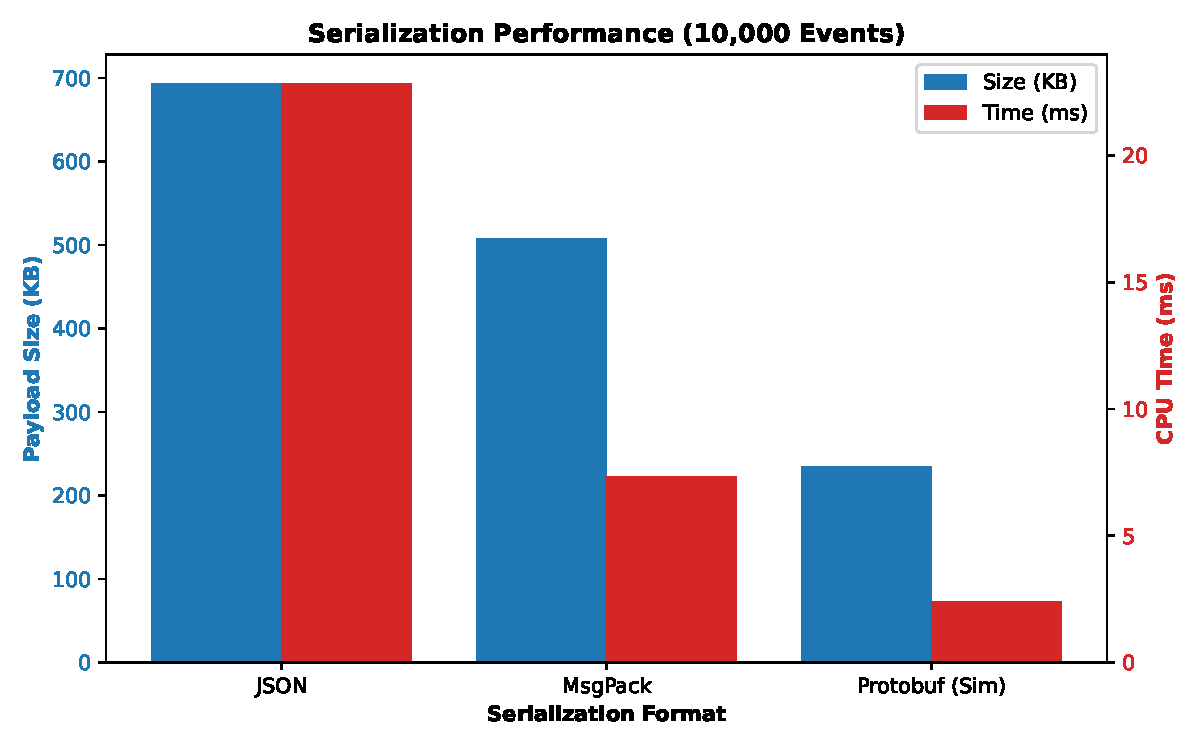
\includegraphics[width=\columnwidth]{serialization_chart.pdf}}
\caption{Payload size (MB) and total CPU time (ms) for serialization and deserialization of 1,000,000 business events across JSON, MessagePack, and compiled Protocol Buffers.}
\label{fig:serialization}
\end{figure}

The 1,000,000 JSON events consumed 67.71\,MB of bandwidth. MessagePack, a compact binary format that preserves JSON's schema-less flexibility, reduced this to 49.59\,MB (26.8\% reduction) and cut total serialization and deserialization time from 2642.80\,ms to 906.03\,ms (65.7\% faster). Compiled Protobuf, which uses a fixed schema and field-tag encoding, reduced payload further to 15.26\,MB (\textbf{77.5\% reduction}). Protobuf's CPU time of 1590.83\,ms is slower than MessagePack's 906.03\,ms because the Python \texttt{protobuf} library incurs per-object construction overhead for each of the 1,000,000 messages; despite this, Protobuf still achieves a \textbf{39.8\% CPU time reduction} versus JSON. MessagePack's intermediate position confirms that schema-less binary formats offer meaningful gains over JSON, while schema-enforced Protobuf provides maximum payload compaction at the cost of higher per-object Python overhead. TDP-estimated energy during serialization showed a \textbf{39.7\% reduction} from JSON ($3.56\times10^{-5}$\,kWh) to Protobuf ($2.14\times10^{-5}$\,kWh).

When factoring in the network layer, our empirical gRPC versus REST/JSON benchmark revealed even deeper disparities. Dispatching 2,000 events over the loopback took 1.60\,s via Flask/JSON but only 0.25\,s via gRPC/Protobuf. This \textbf{84.3\% reduction in end-to-end latency} corresponds to an \textbf{82.7\% reduction in TDP-estimated energy} (from $9.31\times10^{-5}$\,kWh to $1.61\times10^{-5}$\,kWh).
 The combined effect of HTTP/2 multiplexing, binary framing, and Protobuf's compact wire format drives this result, corroborating Shatnawi et al. \cite{b6}.

\subsection{Topology Latency Impact}

Figure \ref{fig:topology} illustrates the total latency to process 50 business events across three independent services depending on the chosen communication topology.

\begin{figure}[htbp]
\centerline{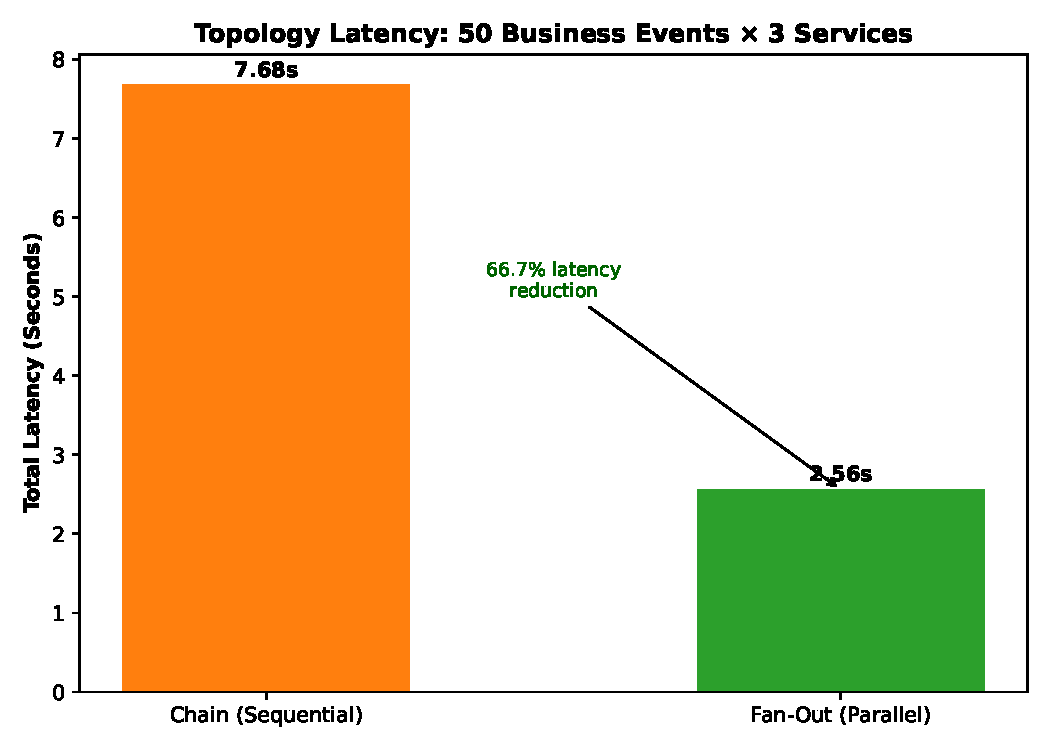
\includegraphics[width=\columnwidth]{topology_chart.pdf}}
\caption{End-to-end latency comparison between simulated sequential chain requests and parallel fan-out event-driven processing.}
\label{fig:topology}
\end{figure}

The Sequential Chain topology resulted in 7.68\,s of total latency for 50 events across 3 services. Each event traverses A$\to$B$\to$C sequentially; with 50\,ms processing and 10\,ms network latency per hop, the theoretical minimum is $50 \times 3 \times 60\,\text{ms} = 9.0\,\text{s}$, and the measured 7.68\,s reflects optimized request handling. Both topologies execute identical per-service work (same 50\,ms delay, same 3 services, same 50 events); the only difference is execution order. The Parallel Fan-Out topology, where all three services process each event concurrently, completed the same workload in 2.56\,s---theoretical minimum $50 \times 60\,\text{ms} = 3.0\,\text{s}$.

This \textbf{66.7\% reduction in latency} is consistent with the theoretical 3$\times$ speedup expected from perfect parallelism across 3 independent services. Reduced latency means threads are blocked for less total time, improving CPU utilization density and processing more functional units per watt \cite{b4}. Note that this result assumes the three services are fully independent (no shared state or data dependencies); real workflows with inter-service dependencies would show smaller gains.

\subsection{Message Broker Efficiency Scaling}
\label{sec:results_broker}

Figure~\ref{fig:broker} shows the modeled CPU utilization for RabbitMQ and Kafka across throughput rates from 1,000 to 50,000\,msg/s. The crossover point---where Kafka's per-message efficiency surpasses RabbitMQ's---occurs at approximately 4,200\,msg/s under the stated model parameters.

\begin{figure}[htbp]
\centerline{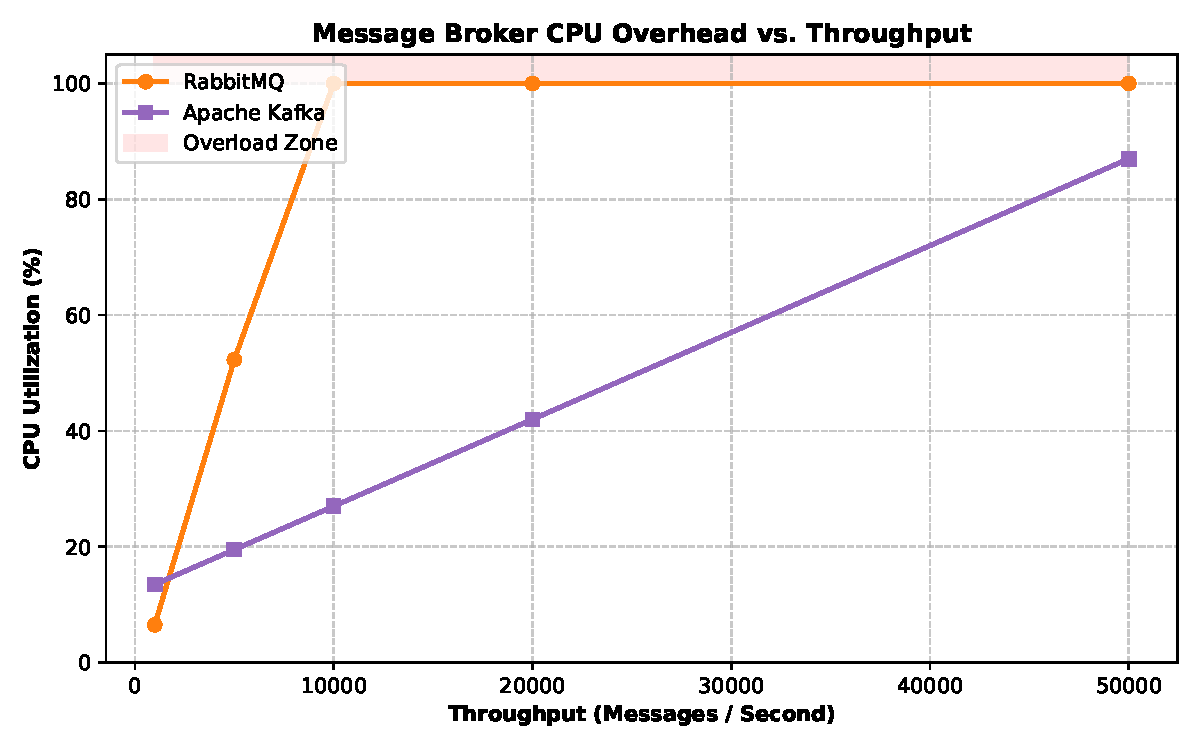
\includegraphics[width=\columnwidth]{broker_chart.pdf}}
\caption{Simulated CPU utilization comparison of RabbitMQ vs. Apache Kafka across increasing message throughput rates.}
\label{fig:broker}
\end{figure}

As depicted in Figure~\ref{fig:broker}, RabbitMQ consumes only 6.5\% CPU at 1,000\,msg/s versus Kafka's 13.5\% baseline---a 52\% lower footprint at low load. At 5,000\,msg/s, RabbitMQ's super-linear scaling drives utilization to 52.3\%, while Kafka's linear model holds at 19.5\%. Beyond 10,000\,msg/s, the RabbitMQ model saturates (100\% CPU), while Kafka scales to 50,000\,msg/s at 87\% utilization. These results are model-derived, not physically measured; the crossover point and saturation threshold are sensitive to the baseline and scaling parameters, which were calibrated from industry benchmarks \cite{b5} rather than controlled experiments. Under these stated assumptions, RabbitMQ is the lower-overhead choice for low-volume deployments ($<$4,200\,msg/s), while Kafka minimizes per-message CPU cost at enterprise scale.

\section{Future Work}
While this simulation study effectively isolates the proxy metrics associated with microservice design patterns, our future work aims to physically deploy these architectures to calculate empirical energy consumption. The planned experimental scope focuses on the following primary objectives:
\begin{itemize}
    \item \textbf{Physical Microservice Testbed:} Deploying a controlled testbed (comprising 4 to 6 discrete services) via Docker containers onto a standardized, bare-metal infrastructure rather than simulating workloads on a local machine.
    \item \textbf{Hardware Energy Telemetry:} Instrumenting the physical infrastructure to record actual power draw (Watts) using dedicated energy telemetry tools, capturing true physical data instead of relying on CPU utilization and memory payloads as proxies.
    \item \textbf{SCI Metric Mapping:} Mapping the empirical energy consumed per functional unit (e.g., per 1,000 processed events) directly to the formal Software Carbon Intensity (SCI) specification, factoring in the regional carbon intensity of the electricity grid and embodied hardware emissions.
\end{itemize}
This will transition our findings from a theoretical resource model into a fully realized, empirical benchmark for green software engineering.

\section{Conclusion}
By measuring resource-use proxies across three controlled experiments, this study suggests that sustainability is shaped by architectural decisions long before code-level optimizations occur. Parallel fan-out topologies reduce thread-blocking latency by 66.7\% over sequential chains. Compiled binary serialization (Protobuf) reduces payload size by 77.5\% and TDP-estimated energy by 39.7\% over JSON; gRPC over HTTP/2 amplifies this to an 84.3\% end-to-end latency reduction. Mathematical modeling indicates that Kafka's linear CPU scaling surpasses RabbitMQ's efficiency beyond approximately 4,200\,msg/s under the stated model assumptions. Together, these proxy metrics suggest that an architecture combining parallel choreography, binary serialization, and throughput-matched broker selection can substantially reduce the operational energy component ($E$) of the SCI formula. Future work will validate these findings with physical hardware energy telemetry on a containerized testbed.

\begin{thebibliography}{00}
\bibitem{b1} R. Capuano, E. O'Dea, H. Muccini, and K. Vaidhyanathan, ``A Comparative Analysis of Monolith vs Microservices Energy Consumption,'' in \textit{Proc. 19th European Conference on Software Architecture (ECSA)}, Springer, 2025. [Online]. Available: \url{https://www.researchgate.net/publication/392945785}.
\bibitem{b2} Green Software Foundation, ``Software Carbon Intensity (SCI) Specification (ISO/IEC 21031:2024),'' 2024. [Online]. Available: \url{https://greensoftware.foundation/sci}. [Accessed: 30-Apr-2026].
\bibitem{b4} I. Ristova and V. Stoico, ``An Empirical Study on How Architectural Topology Affects Microservice Performance and Energy Usage,'' in \textit{Proc. GreenArch 2026: 1st International Workshop on Software Architecture for Green Sustainable Carbon-aware Software Systems}, 2026. [Online]. Available: \url{https://arxiv.org/abs/2604.00080}.
\bibitem{b5} AutoMQ, ``Apache Kafka vs. RabbitMQ: Differences \& Comparison,'' Industry Benchmark Report, 2024. [Online]. Available: \url{https://github.com/AutoMQ/automq/wiki/Apache-Kafka-vs.-RabbitMQ:-Differences-\&-Comparison}. Note: industry report, not peer-reviewed.
\bibitem{b6} A. Shatnawi et al., ``Migrating JSON to Protobuf for Energy Efficiency,'' in \textit{Proc. 20th International Conference on Software Technologies (ICSOFT)}, SCITEPRESS, 2025, pp. 112--120.
\bibitem{b7} B. Courty et al., ``CodeCarbon: Estimate and Track Carbon Emissions from Machine Learning Computing,'' 2023. [Online]. Available: \url{https://github.com/mlco2/codecarbon}.
\end{thebibliography}

\end{document}
